\documentclass[a4paper,titlepage,11pt]{article}
\usepackage{a4wide,graphicx,fancyhdr,amsmath,amssymb,color,hyperref}
\usepackage{enumerate}
\usepackage{listings}
\usepackage[english]{babel}
\usepackage{float}
\usepackage{hyperref}
\usepackage{wrapfig}
%----------------------- Macros and Definitions --------------------------

\setlength\headheight{20pt}
\addtolength\topmargin{-10pt}
\addtolength\footskip{20pt}

\fancypagestyle{plain}{%
	\fancyhf{}
	\fancyfoot[RO,LE]{\sffamily\bfseries\thepage}
	\renewcommand{\headrulewidth}{0pt}
	\renewcommand{\footrulewidth}{1pt}
}

\setcounter{tocdepth}{2}
\setcounter{secnumdepth}{2}

\newcommand{\HRule}{\rule{\linewidth}{0.5mm}}

\newcommand{\uni}{Eindhoven University of Technology}
\newcommand{\fase}{Computer Science and Engineering}
\newcommand{\vak}{Architecture of Distributed Systems}
\newcommand{\vakcode}{2IMN10 }
\newcommand{\essaytitle}{Architecture Comparison of Massive Multiplayer Online Games}
\newcommand{\stad}{Eindhoven}

\pagestyle{fancy}
\fancyhf{}
\fancyhead[R]{\vak}
\fancyhead[L]{\uni}
\fancyfoot[R]{\sffamily\bfseries\thepage}
\fancyfoot[L]{\essaytitle}
\renewcommand{\headrulewidth}{1pt}
\renewcommand{\footrulewidth}{1pt}


\graphicspath{{Images/}}

\author{
	Jasper Selman (0741516) - \texttt{j.w.m.selman@student.tue.nl}
	\and
	Ramon de Vaan (0758873) - \texttt{r.d.vaan@student.tue.nl}
}
\begin{document}

	\begin{titlepage}
	\begin{center}

% Upper part of the page
		
\includegraphics[width=0.15\textwidth]{Images/tuelogo}\\[1cm]

		\textsc{\LARGE \uni}\\[0.2cm]

		\textsc{\fase}\\[1.6cm]

        \textsc{\LARGE \vak}\\[0.5cm]

% Title
\HRule \\[0.4cm]
{ \huge \bfseries \essaytitle}\\[0.4cm]

\HRule \\[1.5cm]

% Author and supervisor
		\begin{minipage}{0.5\textwidth}
			\begin{flushleft} \large
				\emph{Authors:}\\
				Jasper \textsc{Selman} \\
				Ramon \textsc{de Vaan}
			\end{flushleft}
		\end{minipage}

		\vfill

% Bottom of the page
		{\large \today} \\
		\stad

	\end{center}
\end{titlepage} 

	\begin{center}
\section*{Abstract}
\end{center}
Nowadays the gaming industry is one of the most rapidly expanding industries in the world. Especially the multiplayer online games. Due to the vast success of games like World of Warcraft, the amount of vendors of massive multiplayer online games increased, interesting to know therefore is how the architecture of all these games is designed, since this kind of games give a great example of how a distributed architecture works in real life. In this paper we will take a deeper look at this architecture. We will elaborate on the architectural and interaction styles used in the following papers: \emph{Practical Middleware for Massively Multiplayer Online Games} \cite{middleware}, \emph{Requirements of Peer-to-Peer-based Massively Multiplayer Online Gaming} \cite{peer} and \emph{Towards Service Oriented Architecture for MMOG} \cite{service}. We shall also describe how these design choices affect the view of the game state and compare how well the architectures work with respect to performance aspects.\\

	\section{Practical Middleware for Massively Multiplayer Online Games}
The first architecture and it's design choices we are going to review, is the architecture described in \emph{Practical Middleware for Massively Multiplayer Online Games} \cite{middleware}.
In this paper the authors elaborated on the middleware platform. The purpose of such a platform is, how the authors stated it, "Middleware helps programmers manage the complexity and heterogeneity of distributed computing environments". So for short it is a platform which makes it easier to develop and maintain distributed games. The authors have also developed their own platform and have made several architectural design decisions for that. The platform is called Distributed organized Information Terra (DoIT) middleware platform. \\

\begin{wrapfigure}{r}{0.5\textwidth}
\begin{center}
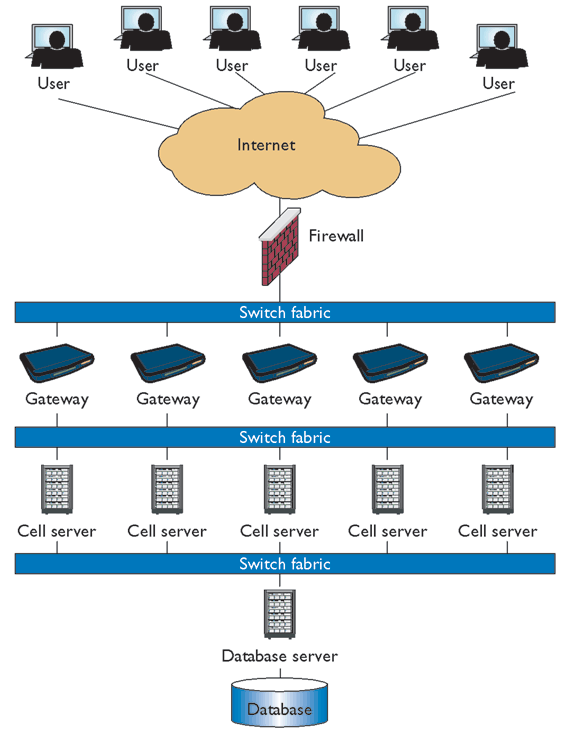
\includegraphics[width=0.4\textwidth]{4tier}
\caption{General framework for middleware platforms for MMOG}
\end{center}
\label{fig:4tier}
\end{wrapfigure}

\noindent A lot of research has been done by researchers to define a framework for middleware platforms. The framework is a 4-tier architecture consisting of a client, a proxy/gateway, a cell server and a database tier. The gamers have control over the client applications. The proxy is in charge of distribution of messages and security aspects. The cell servers maintain the virtual world, it also makes sure that no collisions appear between multiple game clients. The database stores the players states, so that all the changes people made are not wiped clean every time they log off. A graphical view of this architecture is shown in \autoref{fig:4tier} \cite{midfig}. \\
\indent Next to this general framework for the architecture there is also a list of properties which a a middleware platform should adhere to. These properties are \emph{Ease of Development}, \emph{Ease of Deployment}, \emph{Ease of Maintenance}, \emph{Ease of Change} and \emph{Performance and Load Balancing}. For an elaborated description of these properties, we refer to section "Practical Next-Generation MMOG Middleware" in \cite{middleware}.\\

\noindent Now we know the basics of a middleware platform, we shall discuss the architecture of the DoIT platform. This platform uses a message-oriented middleware instead of a RPC-based technology. The authors claim that this of great benefit due to the event-driven behavior of MMOG's. This seems logical. A lot of the game play of MMOG is indeed based on events made by other players. RCP does not really benefit from this, it would be better suited for single player games, because in that case all the procedure calls are done by the one client. \\
\indent Another great advantage of MOM over RCP is that MOM allows decoupling while RCP does not. This is also mentioned by the authors. Next to this difference the DoIT platform differs on two points from the framework mentioned before. The first is that DoIT is customizable and reduces the complexity for MMOG application programmers. The only proof for this, given by the authors, is that a code-generator model is introduced. This model generates message-factory and handler classes for a protocol. The developer still has to define the real detailed content for these handlers. We think that this seems not really enough evidence that this platform really reduces complexity for programmers. It only generates some code automatically (the handlers). The protocol still has to be defined by the programmer and the actual code in the handlers still has to be produced by the programmers. So in practical, the authors only stated that they made a module which generates the handlers for a protocol, but they still have to filled. The only real benefit from this is that you do not forget to create such a handler. So we think this claim is really questionable.\\
\indent The authors also made a small notion of security of their platform. The protocols are modeled as a set of message fields and the generator engine randomly shuffles these fields. This makes hacking specific messages more complicated. The authors also claim with just that this is not really safe yet and that messaging protocols and encryption algorithms are needed to prevent attacks.\\
\indent The last feature DoIT includes is a real-time virtual-world logic, called VWLogic. This logic has as a target to decrease the complexity for the programmers. The idea behind it is really nice. There is a VWLogic adapter which demultiplexes for each VWLogic component, as stated by the authors. When a message comes in, the VWLogic adapter finds the corresponding handler. After that handler is finished the VWLogic adapter sends an update request. Unfortunately the authors do not mention what architecture is used to accomplish this or give any proof of how this works. So the idea is really nice and the programmers certainly benefit from this, if it works.\\

\noindent Another question that comes to mind for these kind of platforms is, how does this architecture affects the game state of a client? This can all be derived from the general framework for middleware which DoIT follows. The MMOG has a central (or multiple, you can play with that a bit) database servers. In these servers the game state of a client is saved. This has as a great advantage that a client user does not depend on the availability of other users (like in a P2P network). The downside of this is that a lot of traffic has to go from/to that database server. \\
The framework tries to minimize this by letting several cell servers interact with this database server. Fortunately this database server does not have to be interacted very often, I assume once to load the clients game state when he logs on and once to store it when he logs of. The massive interaction happens between clients and cell servers. Now I assume that all one cell server handles the game server in which clients are playing or that when several cell servers handle such a game server that they communicate with each other. Otherwise it would not be possible to resolve conflicts between clients, like for instance user A picks up an item and user B picks up the same item at about the same time. This conflict has to be resolved by the client servers. Luckily this can be easily done by doing a request to the server whether this item can be picked up or not. The cell server(s) only allow one of those request. So this client server architecture in the 4-tiered framework ensures that client games are in a steady state.\\
There is now one problem that have to be addressed, that is what happens when one of the cell servers or database servers goes down? When one of the cell servers goes down, than it is possible to distribute the clients over other cell servers. This might affect the performance a bit, due to bigger loads on the other cell servers but it is still better than just dump the connections with the clients that were connected to the failed cell server. A bigger issue is what happens when the database server goes down? Do they have backup servers for that? As shown in the architecture in \cite{midfig} there is only one database server. So when this server is down, the game cannot be played. However we assume that there are (several) backup servers for this database server. In that way the game can still be played.\\
\\
The last part left to discuss is performance of the architecture. We shall discuss some of the above mentioned properties, like maintenance and load distribution, but also properties like security, availability, and scalability. As mentioned before the general architecture of this particular system follows the architecture described in \autoref{fig:4tier}, so we will refer to this figure regarding the properties. The first property we are going to check is maintenance. The authors themselves state "easy maintenance and monitoring are subsequent requirements" in section "Ease of Maintenance" in \cite{middleware}. When we look at the architecture we see that the decoupling of the MOM system makes the maintenance easier for the developers, they do not have to recompile the whole program every time. Also the client server architecture that was provided in \autoref{fig:4tier} shows us that it is possible to do maintenance on some of the client servers. They can do maintenance on some of the servers, while the game still runs on the other servers and when the maintenance is finished they can redistributed the games and maintain the other servers. This can also be done for the database server if they have backup servers. The last part which helps is the VWLogic. When some of the handlers are changed, the VWLogic itself makes sure that the right message is handled by the right handlers. \\
\indent Now let's take a look at the load distribution. This is done quite well via the general middleware architecture. The client runs the graphics, the network communication and the interface, while the servers host the virtual world and handle collisions and the database handles the user state. This can be balanced by spreading the virtual world over multiple servers, or server farms to speed this up. This is also of direct influence on the scalability. If this is done correctly then it is easy to add multiple servers to a cluster or add multiple clusters, or multiple database servers to the entire network. This makes sure that more players can run the game.\\
\indent The security however was not satisfactory as mentioned earlier. There are very few security protocols integrated in the middleware and the authors stated that other security tools/protocols need to be implemented by the vendors themselves. So there is definitely room for improvement in this tool for this, but this can be hard since the correct protocol can depend on the game.\\
\indent The last property is the aspect of availability. This was also briefly discusses before. As long as there are enough (clusters of) servers available for the cell servers, then people can play the game. When one of the servers goes down the load of that server can be redistributed over the other servers. The problem might be in the database server. When that serer is down, the availability of the architecture depends on whether or not (and how many) backup servers are available.



	\section*{Requirements of Peer-to-Peer based Massively Multiplayer Online Gaming}
In the second paper the authors \cite{peer} provide a whole different kind of view on an architecture for MMOG. The peer-to-peer view. Such kind of architecture in its ideal form, reduces the costs made by the game vendor significantly. For example think of the amount of servers which become redundant. The problem with this kind of architecture however is to ensure the consistency and availability of the game. In the next part we will see how well the authors handled these problems. A, not unimportant, note is that the architecture proposed is not yet finished. The authors have ideas how to implement their architecture but this did not happen yet. Therefore the architecture is not complete yet, but we try to reason about all the parts of the architecture for which the ideas are already there.\\
\indent As mentioned before the traditional server-client architecture is very costly, that is why the authors chose for a peer-to-peer architecture. The underlying structure for this peer-to-peer network is going to be a \emph{k-connected network graph}. Such a graph seems very suitable for a peer-to-peer network. When you establish a such a k-connected graph, the properties of it ensures that you are able to remove fewer than $k$ vertices (players) from this graph and the graph is still fully connected. This full connectivity is a must have, because if the graph is not fully connected, people in one part of the graph are not able to receive events which are caused by other players in the other part of the graph. This has the result that these players seem to "freeze" for players in the other part of the network. A difficulty which is not solved by the properties of the k-connected graph is how to add new players to a graph or create a new graph. The authors themselves acknowledge that it is a problem when it is not guaranteed that players are added to an existing graph. Right now the authors are investigating how they can solve this problem. An already proposed solution is the IRC protocol, but we do not really see how this protocol should solve this problem.\\
\indent In contrast to the number of architectural styles there are several interaction styles. The communication middleware used provides two kind of API's. The first supports a reactive world state propagation and the other a proactive world state propagation. The first API is used for activities like virtual crime investigation. The interaction style behind this API is a Request - Reply, or Remote Invocation, style. This style is well suited for this type of activities. The authors themselves give a good example for this: "\emph{if a player is suspected of having acted inappropriately, a game master may actively query the network for all state information about the player's actions in a given time period.}". This also shows us why this interaction style is a terrible choice for the real game play. If the second, proactive, API was also based on this style then all the peers would have to make a request for every action that occurs, this would cause huge delays for the players and as we all know, in MMOG delays are one of the most irritating things that can happen.\\
\indent Luckily the authors had realized that themselves and use a different style for the proactive API. The style behind this API fits best to the event based interaction style, or Indirect Communication style. This seems to be a good choice because the greater part of the communication between peers is based on events in the game caused by other players. A clear problem now was how to distribute all the changes over all the peers. Simply notifying all the peers about every event that happened, even when the event happened miles away, is not a suitable option. So the authors came up with the following solution. The game is partitioned in to a number of sub-areas, called \emph{zones}. In every zone there is one coordinator, which is just a normal peer. Now there are two scenario's. In the first scenario a zone population is sparse. In that case the coordinator observes the peers and determines which peers should exchange events. In the second scenario the zone is densely populated. In that case the coordinator instructs all the peers to stop sending direct messages but instead send everything to the coordinator. The coordinator on its turn sends a message to every other peer in the zone, consisting of a summary of these messages. The authors admit that this is not an ideal solution due to the delay for the update messages but it is an efficient one.\\ 
\indent This style pops some question marks. For example what happens to the game state of a user who is elected as coordinator. The coordinator has substantially more work to do than other peers, does this mean the coordinator has a bigger delay? Also what happens when the coordinator leaves the zone, but it was densely populated and it has not yet send an update message? What happens when a peer is on the edge of a zone and can already see the other zone, does he still only get updates from the zone he is in or also already from the other zone? What happens when a lot of elections of coordinators have to take place due to the unfortunate fact that the newly elected coordinator leaves the game at that time? Does this cause a lot of delay? These are all questions that are very important and unfortunately these cannot be answered yet since the architecture is not yet finished. \\
\indent A whole different problem in this peer-to-peer style, which did not occur in a simple client-server architecture, is the consistency of a game. This is one of the hardest issues in a peer-to-peer network. How do you ensure that the action you just performed is consistent with all the other events in the game? Also another problem is how (and where) do you store all the data when a player logs off? In a client - server you can just store it at a database server, but how do you do this now? The authors acknowledge this problem and think that they can overcome this by interpreting the changes in a game as a series of events. The problem is however how to determine the ordering of these events? A definition of a consistency model has been made, linearizability \cite{linear}. This should help the authors to achieve this ordering. Currently they are investigating how to use this in algorithms to achieve the game consistency.\\
\\
The last part we were going to discuss about the architecture presented in this paper is the performance of it. Think of properties like , maintenance, load distribution, security, availability, usability and scalability. \\
\indent First we take a look at the API's in the communication engine and to which properties these contribute. Likely is that they increase the usability of the engine, since multiple types of games fit in this middleware. The distribution framework gives support for distributed game management and computation, the usability also benefits from this.\\
\indent Next we take a look at the k-connected network. If the authors succeed in implementing this, the availability, reliability and scalability would benefit greatly from it. With such a network the system is able to add people to a network or remove people from it. This represents people logging in and off. If this is possible the system is also able to ensure that the game state of players does not depend on how many other players are online and who goes offline while you are playing. For adding a person to a graph, the authors are currently busy how to add new people to a graph instead of creating a new graph. If and when this works the system is also very well scalable. People could just log in and they are connected to an existing graph.\\
\indent At the moment the authors are also busy investigating how the game world changes have to be distributed over all the peers. If they do this well enough than the load distribution of the game is quite well, but they have to be careful. If the load per peer gets to high, the performance for that single peer might go down a lot. They have also a reactive world state propagation, this propagation is used to do research in virtual crime investigation in the game (which shows us they are thinking about the security of their architecture). Unfortunately we cannot say more about this part since there are no real decisions made yet how to handle this game state changes.\\
\indent The last part the authors are currently busy with tis the consistency of the game. For the game view of the user it is important the game is consistent in such a way that is player A picks up an item, player B cannot pick up this item anymore. At the moment the authors developed a model for ordering of events in a system to be correct, but nothing of this is yet implemented. \\
\indent Overall the system has great potential regarding these performance properties, but it was still in progress so we had to wait for the result how well it is implemented in practice. Since the paper was quite old we tried to find how this peer@play project ended and if it was a success or not, but unfortunately we were not able to find any information on this. So this might insinuate that the architecture in practice was not so good.


	\section*{Towards Service Oriented Architecture for MMOG}
The final architecture we will discuss is the one described in the paper \emph{Towards Service Oriented Architecture for MMOG} \cite{service}.
The main focus of the paper is to propose a service oriented architecture for massive multiplayer online games, that ensures a certain quality of service and provides scalability.
Quality of service mostly seems to be expressed in terms of real-time interaction.
The authors have different measures for real-time interaction, ranging from `non real-time' to `extreme real-time'.
In user communication, the writes attempt to achieve `hard real-time' interaction.
However, some of the other requirements of the system seem to collide with the quality of service requirements. \\

As is apparent from the title, the architecture proposed in the article is aimed at games.
In this case, apart from only focussing on game state, the authors have considered other services in a game as well, for example, the account login service, or the account billing service.
These services are modelled by the service-oriented architecture (SOA) concept.
The SOA ensures functionality like scalability, re-usability, monitoring and tracking of information, and others. \\
Based on this concept, the architecture provides processes for user authentication, user checks, and credit card checks.
These processes are implemented using Business Process Execution Language (BPEL).
BPEL is very well suited to the processes above, while also having a very low deployment cost.
It is even capable of real time services.
However, this is where it clashes with the quality of service requirements. \\
The language can only provide `soft real-time' interaction, one step below the hard real-time interaction we need.
Hence, it does not have the capabilities for peer to peer interaction as far as games go. \\

To solve this, the proposed architecture employs a form of middleware to facilitate peer to peer interactions, separate from the BPEL implementation.
The article proposes the use of an open source `Data Distribution Service (DDS) Standard'.
This standard provides an information hub where users can dynamically connect in order to publish and subscribe to each other's data as needed, in an efficient, high-performance manner, with minimal overhead.
The flexibility of this communication exchange ensures the quality of service requirement.
Additionally, having users publish data to subscribed users themselves saves a lot in terms of needed communication hardware. 
As a result, the proposed system scores very well in the scalability field, since the producer only has to provide the middleware where users can connect to each other. \\

The architecture seems very well thought out in terms of scalability and quality of service.
Splitting the architecture in two parts with slightly different requirements ensures that the system as a whole is more efficient.
The split makes sense, as well.
The SOA concept ensures that the authentication, user check, and credit card check processes remain scalable, with the added benefit that BPEL has a very low deployment cost.
DDS also seems to be very suitable for having users send data to each other. \\

Using DDS says something about how the architecture handles the game state.
Users subscribe to other users for their data, and users publish their data to every user subscribed to them.
However, the article does not state how users are to determine to which users they should subscribe, or what/when they should publish data.
Supposedly, this should be handled by the game engine.
In that manner, each user has it's own portion of the game state, only being subscribed to the users that have data important to that particular user.
This does give rise to some questions regarding security. 
Users may be able to influence the data they send, or just not send data at all. 
All of these might result in inconsistencies in the intersection of game states between users, which might put some users at a disadvantage.\\
However, inconsistencies in the game states do not even have to be deliberate.
Users with a bad internet connection may also affect the game state of other users. 
As per the example given in the article, in a race game, multiple users may think they're at the number one position, due to delayed messages from other players regarding their position on the track.
This may be addressed by game developers, but it does seem like placing a burden upon them, which should actually have been solved in the architecture itself. \\

Now we are going to analyze the architecture proposed in \cite{service} regarding to performance properties like maintenance, load distribution, security, availability, usability and scalability. 
First we would like to discuss the load distribution.
The proposed architecture is split into two parts, where one part is responsible for less network intensive processes, such as user authentication and credit card checks. 
The other part is where the brunt of the communication is done.
With DDS as middleware, the users are able to subscribe to other users for relevant data, and publish data to their own subscribers.
Since DDS only serves as a means for users to subscribe to each other, the load is distributed over all of the users.
As a result, the load is very well distributed, even if the number of users increases, as is common in P2P architectures. 
Moreover, even the other part of the architecture is very open to improvements as needs may change.
The SOA concept calls for loosely coupled entities that are independant.
As such, the system can easily be extended with other services as a chat service.
Thus, even as needs may change in the future, load balancing can still be guaranteed. \\
Now let’s take a closer look at the usability. 
The decoupling discussed above together with the BPEL language proposed in section \emph{Simulation flow in BPEL} of \cite{service} seems to give a great boost for usability. 
The BPEL has great functionality when the processes involved do not have a hard real time constraint. 
It is also stated that this language is a standard for defining processes. 
So this insinuates that there the tool is very usable (usable in the fact that it is easy to use and can model a lot of different processes). 
When there are however a lot of processes involved which do require real time constraints, this solution does not work. 
In that case the authors state that they have to use the DDS standard. 
This standard is open source and dynamic. 
This implies that the system is usable as a middleware system. \\
In terms of availability, the SOA part of the system scores very well.
All of the services are independent of each other, so if one part of the system fails, the others can still function.
In the current implementation, this does not hold much ground, as user authentication is generally a vital part of massive multiplayer online games.
However, if the system was to be extended with a chat server, for example, the game would still be able to function, even if the chat server was unavailable.
Additionally, this helps in maintenance, as several services may be temporarily disabled while updating, without having to shut down the entire game. \\
The availability of the DDS part of the architecture is ambiguous. 
Any user can be disconnected without any problem, the game will still function for the other players.
However, if the DDS server allowing users to subscribe to each other would fail, the structure would crumble.
At first users will still be able to play, as they're already connected to other players.
With the server down, however, they will be unable to connect to new users, so eventually, the game states of each user will become inconsistent. \\

The security of the architecture is not discussed in detail by the article.
It is noted that the SOA concept allows for monitoring and tracking of information.
This could be used to prevent malicious information from entering the services, but in the actual implementation it is not discussed. \\
In the user communication, security is not discussed either.
It seems to be up to the game developers to prevent users from sending malicious data to each other, and to make sure the users connect to the appropriate users.
So overall it is hard to say how secure this architecture is, because this part is not really handled in the paper.\\
The last property we are going to discuss is the scalability.
Obviously, the DDS part of the architecture is highly scalable, as users are only dependant on each other for data, instead of a central server.
The SOA part of the system is also very much scalable. 
It allows for integration of new components, resources, and technologies for system expandability.
This is further confirmed by the fact that the services are loosely coupled, meaning that they are independent.
	\section{Conclusion}

	\begin{thebibliography}{9}

\bibitem{middleware}
	Tsun-Yu Hsiao$\&$ Shyan-Ming Yuan.
	2005.	
 	Practical Middleware for Massively Multiplayer Online Games.
	\emph{IEEE Internet Computing},
	September - October 2005, 47-54.

\bibitem{peer}
	Gregor Schiele, Richard S\"{u}selbeck, Arno Wacker, J\"{o}rg H\"{a}hner, Christian Becker $\&$ Torben Weis.
	2007.	
 	Requiremetns of Peer-to-Peer-based Massively Multiplayer Online Gaming
	\emph{Seventh IEEE International Symposium on Cluster Computing and the Grid}.

\bibitem{service}
	Farrukh Arslan.
	2012.	
 	Towards Serice Oriented Architecture (SOA) for Massive Multiplayer Online Games (MMOG).
	\emph{UKSim},
	82, 538-543.

\bibitem{midfig}
	Tsun-Yu Hsiao$\&$ Shyan-Ming Yuan.
	2005.	
 	Practical Middleware for Massively Multiplayer Online Games.
	\emph{IEEE Internet Computing},
	September - October 2005, 49, figure 1.

\bibitem{linear}
	J. H\"{a}hner, K. Rothermel $\&$ C. Becker.
	2004.	
 	Update-Linearizability: A consistency concept for chronological ordering of events in MANETs. 
	\emph{Proceedings of the 1st IEEE conference on Mobile Ad Hoc and Sensor Systems}.
\end{thebibliography}
\end{document}
